\documentclass[dvipdfmx,10pt]{beamer}
\usetheme{Warsaw}
\usecolortheme[RGB={32, 32, 96}]{structure}
\usefonttheme{professionalfonts}
\setbeamertemplate{navigation symbols}{}
\AtBeginSection[]{
    \frame{\tableofcontents[currentsection, hideallsubsections]}        %目次スライド
}

\usepackage{graphicx}
\usepackage{amsmath, amssymb}
\usepackage{bm}
\usepackage{multicol}
\usepackage{framed}
\usepackage{mathrsfs}
\usepackage{amsfonts}

\usepackage{grffile}
\usepackage{here}
\usepackage{tikz}

\title{第11章\\グリーン関数に対する摂動論}
\author{Ryoi Ohashi}
\date{July 16, 2018}
\institute{Department of Applied Physics, Nagoya University}


\begin{document}

\begin{frame}[plain]
    \maketitle
\end{frame}

\begin{frame}{目的}
    \begin{itemize}
        \item グリーン関数を用いた\textcolor{red}{摂動展開}手法を学ぶ
        \item 熱力学ポテンシャル$\Omega$をグリーン関数より導出する
    \end{itemize}
\end{frame}

\begin{frame}\frametitle{目次}
    \setcounter{tocdepth}{1}
    \tableofcontents
\end{frame}

%==============================================================
\begin{frame}\frametitle{復習}
    ハミルトニアンが$H=H_0+H^{'}$, $\mathscr{H}=H+\mu N$のとき\\
    以下のように定義を行う.
    \begin{block}{1体のグリーン関数}
        \begin{align}
            G_r[u,u'] = -<TA_r(u)A_r^{\dagger}(u')> \tag{1}
        \end{align}
    \end{block}
    \begin{itemize}
        \item $r$は状態を表す指数\\
        \item $A_r^{(\dagger)}(u)$は$a_r^{(\dagger)}$のハイゼンベルグ表示\\
        \item $<X>$は演算子$X$の大正準集団に対する平均
        \begin{align}
            <X>={\rm tr}(X e^{-\beta\mathscr{H}})/{\rm tr}(e^{-\beta\mathscr{H}}) \tag{3}
        \end{align}
        
    \end{itemize}
\end{frame}

\begin{frame}\frametitle{復習}
    $u$に対して$\omega$という量を定義することで, フーリエ級数展開を行える.
    \begin{align}
        G_r[u,u^{'}] = \frac{1}{\beta}\sum_lG_r(i\omega_l)e^{-i\omega_l(u-u^{'})}
    \end{align}
    フェルミ粒子であれば, $\omega_l$は次のような離散的な値をとる.
    \begin{align}
        \omega_l = (2l+1)\pi/\beta,\quad l\in \mathbb{Z}
    \end{align}
\end{frame}

\begin{frame}\frametitle{復習}
    \centering
    \begin{tikzpicture}
        \draw[->] (-3.0,0) -- (3.0,0);
        \draw[->] (0,-3.0) -- (0,3.0);
        \draw[] (0, 2.25) circle (0.1);
        \draw[] (0, 1.75) circle (0.1);
        \draw[] (0, 1.25) circle (0.1);
        \draw[] (0, 0.75) circle (0.1);
        \draw[] (0, 0.25) circle (0.1);
        \draw[] (0,-0.25) circle (0.1);
        \draw[] (0,-0.75) circle (0.1);
        \draw[] (0,-1.25) circle (0.1);
        \draw[] (0,-1.75) circle (0.1);
        \draw[] (0,-2.25) circle (0.1);
        \fill[] ( 2.5,0) circle (0.1);
        \fill[] ( 0.5,0) circle (0.1);
        \fill[] (-0.5,0) circle (0.1);
        \fill[] (-2.5,0) circle (0.1);
        
        \fill[] (2,2) circle (0.1);
        \node[anchor=west] at (2,2) {$E_r$};
        \draw[] (2,1) circle (0.1);
        \node[anchor=west] at (2,1) {$\omega_l$};
    \end{tikzpicture}
\end{frame}

%==============================================================
\section{$T$指数関数および$T$記号の性質}
\begin{frame}
    $U(\beta)$は次のように決まる
    \begin{align}
        e^{-\beta\mathscr{H}}=e^{-\beta\mathscr{H}_0}U(\beta) \tag{7}
    \end{align}
    (8.22)により, $U(\beta)$は摂動展開した形になる
    \begin{align}
        U(\beta) = 1+\sum_{n=1}^{\infty}\frac{(-1)^n}{n!}\int_0^{\beta}P\left[H^{'}(u_1)\cdots H^{'}(u_n)\right]du_1\cdots du_n
    \end{align}
    $P$は{\it Wickの記号}(P.132)である
\end{frame}

\subsection{$T$記号の性質}
\begin{frame}
    \begin{block}{Wickの記号}
        時間の大きさの順に並べる際に, 
        \begin{itemize}
            \centering
            \item 奇数回の置換なら$-$符号
            \item 偶数回の置換なら$+$符号
        \end{itemize}
        をつける
    \end{block}
    \begin{block}{$T$記号}
        時間順序積を示す記号\\
        $a,a^{'}$偶数個でできている演算子$C$について次が成立する
        \begin{align}
            T[C(1),C(2)] &= P[C(2),C(1)] \tag{16} \\
            T[a^{(\dagger)}(1),C(2)] &= T[C(2),a^{(\dagger)}(1)] \tag{17}
        \end{align}
    \end{block}
    \centering
    $H^{'}$が$a,a^{'}$を\textcolor{red}{偶数個含んでいる場合}は,\\ \textcolor{red}{$P$を$T$で置き換えが可能}となる
\end{frame}


%==============================================================
\section{グリーン関数に対する表式}
\begin{frame}
    $U^{-1}(u)$を次のように定める
    \begin{align}
        \left(e^{-u\mathscr{H}}\right)^{-1} = \left(e^{-u\mathscr{H}_0}U(u)\right)^{-1} = U^{-1}(u)e^{u\mathscr{H}_0} \tag{18}
    \end{align}
    これを用いて次の表記を定義する
    \begin{align}
        U(u,u^{'})=U(u)U^{-1}(u^{'}) = T\exp\left[-\int_{u^{'}}^uH^{'}(u_1)du_1\right] \tag{24}
    \end{align}
    以降, $a_r$に対して
    \begin{itemize}
        \item $a_r(u) = e^{u\mathscr{H}_0}a_re^{-u\mathscr{H}_0}$ : 相互作用表示
        \item $A_r(u) = e^{u\mathscr{H}}a_re^{-u\mathscr{H}}$ : ハイゼンベルグ表示
    \end{itemize}
    と表記する
\end{frame}

\begin{frame}
    グリーン関数をこの$U(\beta)$を用いて変形する
    \begin{block}{Recall}
        \begin{align}
            G_r[u,u'] = -<TA_r(u)A_r^{\dagger}(u')> \tag{1}
        \end{align}
    \end{block}
    $u>u^{'}$と仮定すると
    \begin{align*}
        G_r[u,u'] &= {\rm tr}(e^{-\beta\mathscr{H}}A_r(u)A_r^{\dagger}(u'))/{\rm tr}(e^{-\beta\mathscr{H}})\nonumber\\
        &= {\rm tr}(e^{-\beta\mathscr{H}}A_r(u)A_r^{\dagger}(u'))/Z_{G0}<U(\beta)>_0 \nonumber
    \end{align*}
    分子について
    \begin{align*}
        &{\rm tr}(e^{-\beta\mathscr{H}}A_r(u)A_r^{\dagger}(u')) = {\rm tr}(e^{-\beta\mathscr{H}_0}U(\beta,u)a_r(u)U(u,u^{'})a_r^{\dagger}(u')U(u^{'},0)) \nonumber\\
        &= {\rm tr}\left(e^{-\beta\mathscr{H}_0}T\left[\exp\left\{-\int_0^{\beta}H^{'}(u_1)du_1\right\}a_r(u)a_r^{\dagger}(u^{'})\right]\right) \tag{27}
    \end{align*}
\end{frame}
\begin{frame}
    \begin{block}{グリーン関数}
        \begin{align*}
            G_r[u,u^{'}] = -\frac{\left<T\left[\exp\left\{-\int_0^{\beta}H^{'}(u_1)du_1\right\}a_r(u)a_r^{\dagger}(u^{'})\right]\right>_0}{\left<T\left[\exp\left\{-\int_0^{\beta}H^{'}(u_1)du_1\right\}\right]\right>_0} \tag{28}
        \end{align*}
    \end{block}
    この結果は$u>u^{'}$と同様に$u<u^{'}$でも成立する\\
    記号的に次のような表記もする
    \begin{block}{}
        \begin{align*}
            G_r[u,u^{'}] = \frac{-\left<TU(\beta)a_r(u)a_r^{\dagger}(u^{'})\right>_0}{\left<U(\beta)\right>_0} \tag{29}
        \end{align*}
    \end{block}
\end{frame}


%==============================================================
\section{グリーン関数に対するファインマン図形}
\begin{frame}
    グリーン関数はフーリエの形で次のようになる
    \begin{block}{}
        \begin{align}
            G_r[u,u^{'}] = \frac{1}{\beta}\sum_lG_r(i\omega_l)e^{-i\omega_l(u-u^{'})}
        \end{align}
    \end{block}
    \centering
    この時の$G_r(i\omega)$はどのように求めるのか?\\
    
\begin{tikzpicture}
        \draw[->, very thick,red] (0.0,0.5) -- (0.0,-0.5);
    \end{tikzpicture}\\
    次のページの順序に従うと計算可能!
    
\end{frame}

\subsection{$G_r(i\omega_l)$の計算の規則}
\begin{frame}{計算手順}
    % \small
    \footnotesize
    \begin{enumerate}
        \item \textcolor{red}{外線}とつながった$n$次のすべての可能なファインマン図形を描く
        \item そのような図形に次の式を当てはめる
        \begin{align*}
            \frac{(-1)^n(-1)^{n_l}}{n!(2\beta V)^n}\prod_{i=1}^{n}\left(r_is_i|v|r_i's_i'\right)
        \end{align*}
        \item $r$, $l$の電子線に次の式を対応させる
        \begin{align*}
            g_r(i\omega_l) = (i\omega_l-\varepsilon_r)^{-1}
        \end{align*}
        同時刻の場合は
        \begin{align*}
            (i\omega_l-\varepsilon_r)^{-1}\exp(i\omega_l0)
        \end{align*}
        \item エネルギー保存則を考慮する
        \begin{align*}
            \omega_{l_1} + \omega_{l_2} = \omega_{l_3} + \omega_{l_4}
        \end{align*}
        \item 外線の$r$,$l$は固定し, 他の変数に関して和をとる
    \end{enumerate}
    \normalsize
\end{frame}

\begin{frame}{外線}
    \begin{block}{外線とは}
        \centering
        $u'$から出ている線, 及び$u$に入る線
    \end{block}
    \centering
    \begin{tikzpicture}
        \node[anchor=east] at (-5.0,-1.0) {$u'$};
        \draw[->,thick,red] (-5.0,-1.0) -- (-5.0, 0.0);
        \draw[-, thick,red] (-5.0, 0.0) -- (-5.0, 1.0);
        \node[anchor=east] at (-5.0, 1.0) {$u$};
        \draw[->,thick] (-3.0,-1.0) arc (-90:90:1);
        \draw[->,thick] (-3.0, 1.0) arc (90:270:1);
        \draw[dashed, thick] (-4.0, 0.0) -- (-2.0, 0.0);
        \node[anchor=north] at (-3.5,-1.5) {つながらない図形};

        \node[anchor=east] at ( 1.0,-1.0) {$u'$};
        \draw[->,thick,red] ( 1.0,-1.0) -- ( 1.5,-0.5);
        \draw[-,thick,red] ( 1.5,-0.5) -- ( 2.0, 0.0);
        \draw[->, thick,red] ( 2.0, 0.0) -- ( 1.5, 0.5);
        \draw[-, thick,red] ( 1.5, 0.5) -- ( 1.0, 1.0);
        \node[anchor=east] at ( 1.0, 1.0) {$u$};
        \draw[->,thick] ( 3.5, 0.5) arc (90:450:0.5);
        \draw[dashed, thick] ( 2.0, 0.0) -- ( 3.0, 0.0);
        \node[anchor=north] at ( 2.5,-1.5) {つながった図形};
    \end{tikzpicture}
\end{frame}

\begin{frame}{例:1次でのファインマン図}
    図8.2より一次のファインマン図は次の二通り\\
    \centering
    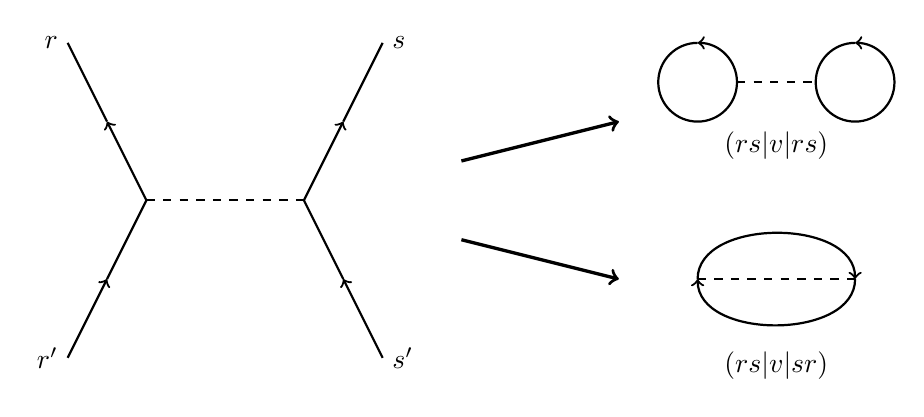
\begin{tikzpicture}

        \node[anchor=east] at (-6.0,-2.0) {$r'$};
        \draw[->,thick] (-6.0,-2.0) -- (-5.5,-1.0);
        \draw[-,thick] (-5.5,-1.0) -- (-5.0, 0.0);
        \draw[->, thick] (-5.0, 0.0) -- (-5.5, 1.0);
        \draw[-, thick] (-5.5, 1.0) -- (-6.0, 2.0);
        \node[anchor=east] at (-6.0, 2.0) {$r$};
        \draw[dashed, thick] (-5.0, 0.0) -- (-3.0, 0.0);
        \node[anchor=west] at (-2.0,-2.0) {$s'$};
        \draw[->,thick] (-2.0,-2.0) -- (-2.5,-1.0);
        \draw[-,thick] (-2.5,-1.0) -- (-3.0, 0.0);
        \draw[->, thick] (-3.0, 0.0) -- (-2.5, 1.0);
        \draw[-, thick] (-2.5, 1.0) -- (-2.0, 2.0);
        \node[anchor=west] at (-2.0, 2.0) {$s$};
        
        \draw[->, very thick] (-1.0, 0.5) -- ( 1.0, 1.0);
        \draw[->, very thick] (-1.0,-0.5) -- ( 1.0,-1.0);

        \draw[->,thick] ( 2.0, 2.0) arc (90:450:0.5);
        \draw[dashed, thick] ( 2.5, 1.5) -- ( 3.5, 1.5);
        \draw[->,thick] ( 4.0, 2.0) arc (90:450:0.5);
        \node[anchor=north] at ( 3.0, 1.0) {$(rs|v|rs)$};

        \draw[->,thick] ( 2.0,-1.0) to [out=90, in=90] ( 4.0,-1.0);
        \draw[dashed, thick] ( 2.0,-1.0) -- ( 4.0,-1.0);
        \draw[->,thick] ( 4.0,-1.0) to [out=-90, in=-90] ( 2.0,-1.0);
        \node[anchor=north] at ( 3.0,-1.8) {$(rs|v|sr)$};
    \end{tikzpicture}
\end{frame}

\begin{frame}{例:1次でのファインマン図}
    片方の線を外線と結ぶように開く\\
    \centering
    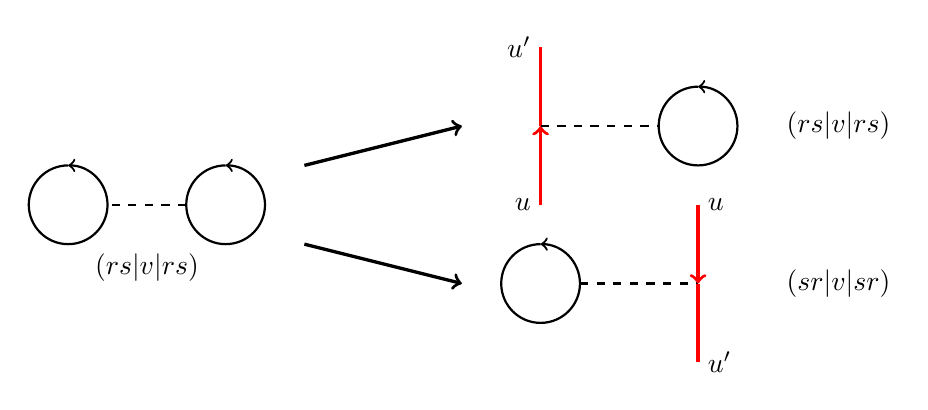
\begin{tikzpicture}
        \draw[->,thick] (-2.0, 0.5) arc (90:450:0.5);
        \draw[dashed, thick] (-2.5, 0.0) -- (-3.5, 0.0);
        \draw[->,thick] (-4.0, 0.5) arc (90:450:0.5);
        \node[anchor=north] at (-3.0,-0.5) {$(rs|v|rs)$};

        \draw[->, very thick] (-1.0, 0.5) -- ( 1.0, 1.0);
        \draw[->, very thick] (-1.0,-0.5) -- ( 1.0,-1.0);

        \node[anchor=east] at ( 2.0, 0.0) {$u$};
        \draw[->,very thick,red] ( 2.0, 0.0) -- ( 2.0, 1.0);
        \draw[-, very thick,red] ( 2.0, 1.0) -- ( 2.0, 2.0);
        \node[anchor=east] at ( 2.0, 2.0) {$u'$};
        \draw[dashed, thick] ( 2.0, 1.0) -- ( 3.5, 1.0);
        \draw[->,thick] ( 4.0, 1.5) arc (90:450:0.5);
        \node[anchor=west] at ( 5.0, 1.0) {$(rs|v|rs)$};

        \draw[->,thick] ( 2.0,-0.5) arc (90:450:0.5);
        \draw[dashed, thick] ( 2.5,-1.0) -- ( 4.0,-1.0);
        \node[anchor=west] at ( 4.0,-2.0) {$u'$};
        \draw[->,very thick,red] ( 4.0, 0.0) -- ( 4.0,-1.0);
        \draw[-, very thick,red] ( 4.0,-1.0) -- ( 4.0,-2.0);
        \node[anchor=west] at ( 4.0, 0.0) {$u$};
        \node[anchor=west] at ( 5.0,-1.0) {$(sr|v|sr)$};
    \end{tikzpicture}
    閉じた図形の数は$n_l=1$
\end{frame}

\begin{frame}{例:1次でのファインマン図}
    片方の線を外線と結ぶように開く\\
    \centering
    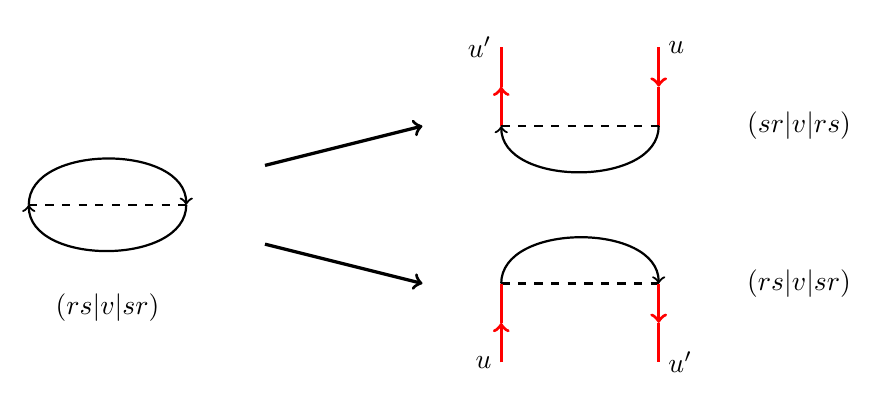
\begin{tikzpicture}
        \draw[->,thick] (-4.0, 0.0) to [out=90, in=90] (-2.0, 0.0);
        \draw[dashed, thick] (-4.0, 0.0) -- (-2.0, 0.0);
        \draw[->,thick] (-2.0, 0.0) to [out=-90, in=-90] (-4.0, 0.0);
        \node[anchor=north] at (-3.0,-1.0) {$(rs|v|sr)$};

        \draw[->, very thick] (-1.0, 0.5) -- ( 1.0, 1.0);
        \draw[->, very thick] (-1.0,-0.5) -- ( 1.0,-1.0);

        \node[anchor=west] at ( 4.0, 2.0) {$u$};
        \draw[->,very thick, red] ( 2.0, 1.0) -- ( 2.0, 1.5);
        \draw[-,very thick, red] ( 2.0, 1.5) -- ( 2.0, 2.0);
        \draw[->,very thick, red] ( 4.0, 2.0) -- ( 4.0, 1.5);
        \draw[-,very thick, red] ( 4.0, 1.5) -- ( 4.0, 1.0);
        \node[anchor=east] at ( 2.0, 2.0) {$u'$};
        \draw[dashed, thick] ( 2.0, 1.0) -- ( 4.0, 1.0);
        \draw[->,thick] ( 4.0, 1.0) to [out=-90, in=-90] ( 2.0, 1.0);
        \node[anchor=west] at ( 5.0, 1.0) {$(sr|v|rs)$};

        \draw[->,thick] ( 2.0,-1.0) to [out=90, in=90] ( 4.0,-1.0);
        \draw[dashed, thick] ( 2.0,-1.0) -- ( 4.0,-1.0);
        \node[anchor=east] at ( 2.0,-2.0) {$u$};
        \draw[->,very thick, red] ( 2.0,-2.0) -- ( 2.0,-1.5);
        \draw[-,very thick, red] ( 2.0,-1.5) -- ( 2.0,-1.0);
        \draw[->,very thick, red] ( 4.0,-1.0) -- ( 4.0,-1.5);
        \draw[-,very thick, red] ( 4.0,-1.5) -- ( 4.0,-2.0);
        \node[anchor=west] at ( 4.0,-2.0) {$u'$};
        \node[anchor=west] at ( 5.0,-1.0) {$(rs|v|sr)$};
    \end{tikzpicture}
    閉じた図形の数は$n_l=0$
\end{frame}

\begin{frame}{計算手順(Remind)}
    % \small
    \footnotesize
    \begin{enumerate}
        \item 外線とつながった$n$次のすべての可能なファインマン図形を描く
        \item そのような図形に次の式を当てはめる
        \begin{align*}
            \frac{(-1)^n(-1)^{n_l}}{n!(2\beta V)^n}\prod_{i=1}^{n}\left(r_is_i|v|r_i's_i'\right)
        \end{align*}
        \item \underline{$r$, $l$の電子線に次の式を対応させる}
        \begin{align*}
            \underline{g_r(i\omega_l) = (i\omega_l-\varepsilon_r)^{-1}}
        \end{align*}
        \underline{同時刻の場合は}
        \begin{align*}
            \underline{(i\omega_l-\varepsilon_r)^{-1}\exp(i\omega_l0)}
        \end{align*}
        \textcolor{red}{$\rightarrow$どの図形が当てはまる?}
        \item エネルギー保存則を考慮する
        \begin{align*}
            \omega_{l_1} + \omega_{l_2} = \omega_{l_3} + \omega_{l_4}
        \end{align*}
        \item 外線の$r$,$l$は固定し, 他の変数に関して和をとる
    \end{enumerate}
    \normalsize
\end{frame}

\begin{frame}{図形と式の当てはめ方}
    \centering
    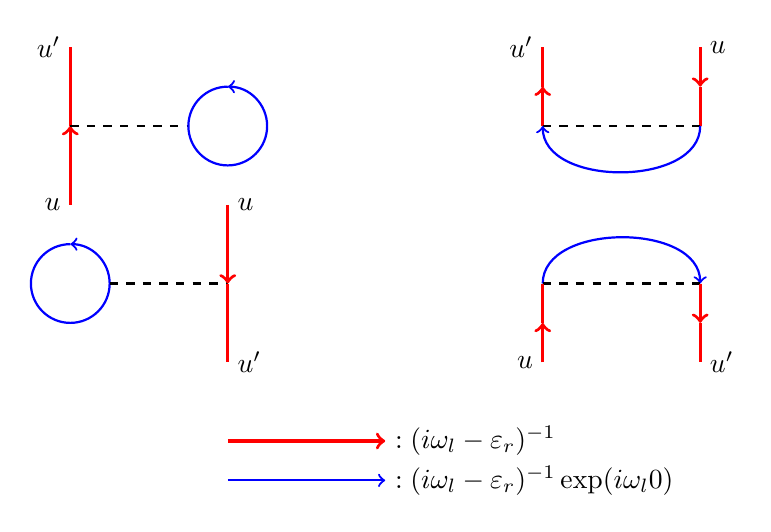
\begin{tikzpicture}
        \node[anchor=east] at (-4.0, 0.0) {$u$};
        \draw[->,very thick,red] (-4.0, 0.0) -- (-4.0, 1.0);
        \draw[-, very thick,red] (-4.0, 1.0) -- (-4.0, 2.0);
        \node[anchor=east] at (-4.0, 2.0) {$u'$};
        \draw[dashed, thick] (-4.0, 1.0) -- (-2.5, 1.0);
        \draw[->,thick,blue] (-2.0, 1.5) arc (90:450:0.5);

        \draw[->,thick,blue] (-4.0,-0.5) arc (90:450:0.5);
        \draw[dashed, thick] (-3.5,-1.0) -- (-2.0,-1.0);
        \node[anchor=west] at (-2.0,-2.0) {$u'$};
        \draw[->,very thick,red] (-2.0, 0.0) -- (-2.0,-1.0);
        \draw[-, very thick,red] (-2.0,-1.0) -- (-2.0,-2.0);
        \node[anchor=west] at (-2.0, 0.0) {$u$};

        \node[anchor=west] at ( 4.0, 2.0) {$u$};
        \draw[->,very thick, red] ( 2.0, 1.0) -- ( 2.0, 1.5);
        \draw[-,very thick, red] ( 2.0, 1.5) -- ( 2.0, 2.0);
        \draw[->,very thick, red] ( 4.0, 2.0) -- ( 4.0, 1.5);
        \draw[-,very thick, red] ( 4.0, 1.5) -- ( 4.0, 1.0);
        \node[anchor=east] at ( 2.0, 2.0) {$u'$};
        \draw[dashed, thick] ( 2.0, 1.0) -- ( 4.0, 1.0);
        \draw[->,thick,blue] ( 4.0, 1.0) to [out=-90, in=-90] ( 2.0, 1.0);

        \draw[->,thick,blue] ( 2.0,-1.0) to [out=90, in=90] ( 4.0,-1.0);
        \draw[dashed, thick] ( 2.0,-1.0) -- ( 4.0,-1.0);
        \node[anchor=east] at ( 2.0,-2.0) {$u$};
        \draw[->,very thick, red] ( 2.0,-2.0) -- ( 2.0,-1.5);
        \draw[-,very thick, red] ( 2.0,-1.5) -- ( 2.0,-1.0);
        \draw[->,very thick, red] ( 4.0,-1.0) -- ( 4.0,-1.5);
        \draw[-,very thick, red] ( 4.0,-1.5) -- ( 4.0,-2.0);
        \node[anchor=west] at ( 4.0,-2.0) {$u'$};

        \draw[->, very thick, red] (-2.0,-3.0) -- ( 0.0,-3.0);
        \node[anchor=west] at ( 0.0,-3.0) {$:(i\omega_l-\varepsilon_r)^{-1}$};
        \draw[->, thick, blue] (-2.0,-3.5) -- ( 0.0,-3.5);
        \node[anchor=west] at ( 0.0,-3.5) {$:(i\omega_l-\varepsilon_r)^{-1}\exp(i\omega_l0)$};
    \end{tikzpicture}
\end{frame}

\begin{frame}
    この手順に従った結果が次の通り
    \begin{block}{$G_r(i\omega_l)$の1次の寄与}
        \begin{align*}
            \frac{1}{2\beta V}\frac{1}{(i\omega_l-\varepsilon_r)^2}\sum_{sm}\left[(rs|v|rs)+(sr|v|sr)\right.\\
            \left.-(rs|v|sr)-(sr|v|rs)\right]\frac{\exp(i\omega_m 0)}{i\omega_m-\varepsilon_s} \tag{47}
        \end{align*}
    \end{block}
    この方法を$n=2,3,\cdots$と次数を増やした場合でも計算していくことで, $G_r(i\omega_l)$を求めることが可能
\end{frame}

%==============================================================
\section{自己エネルギー(self-energy)}
\begin{frame}
    hello
\end{frame}

%==============================================================
\section{電子ガスへの応用}
\subsection{リング近似との関係}
\begin{frame}
    hello
\end{frame}

\end{document}